\documentclass{sigchi}

% Use this section to set the ACM copyright statement (e.g. for
% preprints).  Consult the conference website for the camera-ready
% copyright statement.

% Copyright
\CopyrightYear{2016}
%\setcopyright{acmcopyright}
\setcopyright{acmlicensed}
%\setcopyright{rightsretained}
%\setcopyright{usgov}
%\setcopyright{usgovmixed}
%\setcopyright{cagov}
%\setcopyright{cagovmixed}
% DOI
\doi{http://dx.doi.org/10.475/123_4}
% ISBN
\isbn{123-4567-24-567/08/06}
%Conference
\conferenceinfo{CHI'16,}{May 07--12, 2016, San Jose, CA, USA}
%Price
\acmPrice{\$15.00}

% Use this command to override the default ACM copyright statement
% (e.g. for preprints).  Consult the conference website for the
% camera-ready copyright statement.

%% HOW TO OVERRIDE THE DEFAULT COPYRIGHT STRIP --
%% Please note you need to make sure the copy for your specific
%% license is used here!
% \toappear{
% Permission to make digital or hard copies of all or part of this work
% for personal or classroom use is granted without fee provided that
% copies are not made or distributed for profit or commercial advantage
% and that copies bear this notice and the full citation on the first
% page. Copyrights for components of this work owned by others than ACM
% must be honored. Abstracting with credit is permitted. To copy
% otherwise, or republish, to post on servers or to redistribute to
% lists, requires prior specific permission and/or a fee. Request
% permissions from \href{mailto:Permissions@acm.org}{Permissions@acm.org}. \\
% \emph{CHI '16},  May 07--12, 2016, San Jose, CA, USA \\
% ACM xxx-x-xxxx-xxxx-x/xx/xx\ldots \$15.00 \\
% DOI: \url{http://dx.doi.org/xx.xxxx/xxxxxxx.xxxxxxx}
% }

% Arabic page numbers for submission.  Remove this line to eliminate
% page numbers for the camera ready copy
% \pagenumbering{arabic}

% Load basic packages
\usepackage{balance}       % to better equalize the last page
\usepackage{graphics}      % for EPS, load graphicx instead 
\usepackage[T1]{fontenc}   % for umlauts and other diaeresis
\usepackage{txfonts}
\usepackage{mathptmx}
\usepackage[pdflang={en-US},pdftex]{hyperref}
\usepackage{color}
\usepackage{booktabs}
\usepackage{textcomp}
\usepackage{subcaption}
\usepackage{graphicx}
\usepackage[toc,page]{appendix}
% \usepackage{tikz}
%\def\checkmark{\tikz\fill[scale=0.4](0,.35) -- (.25,0) -- (1,.7) -- (.25,.15) -- cycle;} 

% Some optional stuff you might like/need.
\usepackage{microtype}        % Improved Tracking and Kerning
% \usepackage[all]{hypcap}    % Fixes bug in hyperref caption linking
\usepackage{ccicons}          % Cite your images correctly!
% \usepackage[utf8]{inputenc} % for a UTF8 editor only

% Packages
\usepackage[table,xcdraw]{xcolor}
\usepackage{enumitem}
%\usepackage{booktabs,caption}
\usepackage{tabularx}
\usepackage[flushleft]{threeparttable}

% % Creating a custom itemize
% \setlistdepth{5}

% \newlist{longitem}{itemize}{5}
% \setlist[longitem,1]{label={--}}
% \setlist[longitem,2]{label={--}}
% \setlist[longitem,3]{label={--}}
% \setlist[longitem,4]{label={--}}
% \setlist[longitem,5]{label={--}}

% Custom column type for tabularx environment. Centers and fills
\newcolumntype{Y}{>{\centering\arraybackslash}X}

% Paper metadata (use plain text, for PDF inclusion and later
% re-using, if desired).  Use \emtpyauthor when submitting for review
% so you remain anonymous.
\def\plaintitle{Tap pressure on touchscreens and the relationship to detection of emotion}
\def\plainauthor{First Author, Second Author, Third Author,
  Fourth Author, Fifth Author, Sixth Author}
\def\emptyauthor{}
\def\plainkeywords{Human centered multimedia; emotion; tap pressure}
\def\plaingeneralterms{Documentation, Standardization}

% llt: Define a global style for URLs, rather that the default one
\makeatletter
\def\url@leostyle{%
  \@ifundefined{selectfont}{
    \def\UrlFont{\sf}
  }{
    \def\UrlFont{\small\bf\ttfamily}
  }}
\makeatother
\urlstyle{leo}

% To make various LaTeX processors do the right thing with page size.
\def\pprw{8.5in}
\def\pprh{11in}
\special{papersize=\pprw,\pprh}
\setlength{\paperwidth}{\pprw}
\setlength{\paperheight}{\pprh}
\setlength{\pdfpagewidth}{\pprw}
\setlength{\pdfpageheight}{\pprh}

% Make sure hyperref comes last of your loaded packages, to give it a
% fighting chance of not being over-written, since its job is to
% redefine many LaTeX commands.
\definecolor{linkColor}{RGB}{6,125,233}
\hypersetup{%
  pdftitle={\plaintitle},
% Use \plainauthor for final version.
%  pdfauthor={\plainauthor},
  pdfauthor={\emptyauthor},
  pdfkeywords={\plainkeywords},
  pdfdisplaydoctitle=true, % For Accessibility
  bookmarksnumbered,
  pdfstartview={FitH},
  colorlinks,
  citecolor=black,
  filecolor=black,
  linkcolor=black,
  urlcolor=linkColor,
  breaklinks=true,
  hypertexnames=false
}

% create a shortcut to typeset table headings
% \newcommand\tabhead[1]{\small\textbf{#1}}

% End of preamble. Here it comes the document.
\begin{document}

\title{\plaintitle}

\numberofauthors{1}
  \author{
  \alignauthor Kevin Blom\\
         \affaddr{University of Amsterdam}\\
         \affaddr{Science Park 904}\\
         \email{xxxxxx@xxxxxx.xx}
  }
\maketitle

\begin{abstract}
  % UPDATED---\today. This sample paper describes the formatting
  % requirements for SIGCHI conference proceedings, and offers
  % recommendations on writing for the worldwide SIGCHI
  % readership. Please review this document even if you have submitted
  % to SIGCHI conferences before, as some format details have changed
  % relative to previous years. Abstracts should be about 150 words and
  % are required.
\end{abstract}

\category{H.5.2.}{Information Interfaces and Presentation}{User-centered design}

\keywords{\plainkeywords}

\section{Introduction} % (fold)
\label{sec:introduction}
Affective computing as introduced by Picard\cite{Picard1995} in 1995 lays a foundation for computers and technology to incorporate the recognition and expression of emotions. It can provide better performance when assisting humans or enhance the computers ability to make decisions. It does not have the goal of making computers more human-like, but it is more practical in nature; make computers function with intelligence and sensitivity towards its users\cite{Picard1997}.  According to Shah et al.\cite{Shah2015} there are two general models to represent emotion; discrete and continuous. The discrete model represent emotions that are measurable and physiologically distinct like angry, sad, happy, etc. \cite{Ekman1992} The continuous model represents emotions on a two-dimensional scale, where one axis represents \textit{valence} and the other \textit{arousal} \cite{Posner2005}. Mauss et al. \cite{Mauss2009} suggest that using a dimensional framework is a better option when capturing emotion, relative to discrete frameworks. Since, the measuring of emotion has been a subject of research and several different angles have been discovered to approach it.

\subsection{Physiological detection} % (fold)
\label{sub:physiology}
One angle uses physiological signals of the human body to measure and detect emotion. In a review by Wioleta\cite{Wioleta2013}, eight studies were collected that measure emotion using one or more physiological signals combined. These signals are \textit{EEG, skin conductance, blood volume pulse, temperature, heart rate, blood pressure, respiration, EMG,} and \textit{ECG}. Most of these physiological signals have the drawback that they need specialized sensors attached to the body, making unobtrusive measurements difficult. With the recent rise of smart wearables, heart rate is one of the signals that is more readily available to use in applications on smart devices.
% subsection physiology (end)

\subsection{Facial detection} % (fold)
\label{sub:facial_detection}
Facial detection of emotion incorporates the measurement of facial muscle movement, voice or speech \cite{Ververidis2004}, and also includes the eye as point of detection, i.e. movement, blinking, and pupil dilation \cite{Soleymani2015}. By connecting facial muscle movement to visual display of emotions, Ekman et al. \cite{Ekman1969} conclude with a basic set of six mutually exclusive emotions that could be recognized. Expanding, De Silva et al. \cite{Silva1997} found that several emotions are expressed by either visual or auditory cues, or both, meaning that some emotions can be recognized by visual cues alone, auditory cues alone, or need a combination of both to be detected accurately.
% subsection facial_emotion_detection (end)

\subsection{Posture/gestures emotion detection}
Other means of detection emotions involve the tracking and interpretation of posture and gesture. Wallbott et al. \cite{Wallbott1998} concluded in 1998 that there are, in some cases, distinctive patterns of movement and postural behavior that have a strong correlation to emotions. In other cases, they mention that in absence of patterns there are still distinctive features from which emotion could be inferred. Coulson et al. \cite{Coulson2004} researched static body postures and the recognition of emotions from these body postures by participants. It showed that disgust is a tough emotion to recognize but anger and sadness had over 90\% correct detection rates. Furthermore, happiness and surprise were two emotions that were often confused. 

\subsection{Practical applications} % (fold)
\label{sub:practical_applications}
Looking at a more practical and applied side of emotion detection, Gao et al. \cite{Gao2012} used touchscreen devices, where the application of gestures on touch screens was successfully linked to emotional states with the use of a game. The emotional states that were tested for are: excited, relaxed, frustrated and bored, and accuracy of detection reached at minimum 69\%. However, the research of Gao et al. was limited to gestures and did not incorporate data from taps. Furthermore, Lv et al. \cite{H.R.LvZ.L.LinW.J.Yin2008} have created means to detect emotion from keyboard pressure using feature extraction. This indicates that the use of a keyboard on a touch screen could also be used as means of detecting emotion, but one must keep in mind that a regular keyboard is not fully comparable to a touchscreen keyboard. It lays flat on a desk, and is often typed upon with more than one or two fingers, which means that the pressure exerted on the keyboard is likely not directly correlated with the pressure on a touchscreen keyboard. Moreover, Lee et al \cite{Lee2012} propose an unobtrusive way of detecting emotion by analyzing smartphone usage patterns (not unlike LiKamWa et al. \cite{Likamwa2013}) and social network status updates. However, this required that the user would post status updates through independently developed social networking applications, that are not officially supported by the social networks themselves.

% subsection practical_applications (end)

\subsection{Research Question}
From the related work can be concluded that most types of detection of emotions are invasive, either requiring constant monitoring, possibly with sensors attached to the body, or by constant recording of audio and visual data. The touch screen is a technology a lot of people interact with every day, where they deliberately choose to participate in those interactions. Using touch screen presses as indicators for emotional state could be an unobtrusive way of detecting emotion without the need for constant monitoring. With the introduction of pressure sensitive touchscreens in recent smart devices, an interesting new sensor is added to the plethora of sensors already available. Subsequently, this leads to the following research question:\\

\textit{Can pressure sensitive touch screen devices be used to tell more about the mood of the user?}\\
% \begin{itemize}
%   \item Description of background.
%   \item Explanation of why research was necessary.
%   \item Description of how research will be undertaken.
% \end{itemize}

% section Introduction (end)

\section{Methods} % (fold)
\label{sec:methods}
In order to test for the correlation between taps on a touch screen and emotion, there has to be a standardized way of eliciting different emotions. Fortunately, there exists a photo set that has been thoroughly tested for emotional response on a two dimensional scale that is called the Geneva Affective Picture Database (GAPED) \cite{Dan-glauser2011}. Utilizing the emotional responses of this photo set as a baseline, touch screen taps and their pressure can be compared to emotional response.
Participants were selected using a convience sampling process at an office. The participants varied in age, educational level, current line of work, and background.

\subsection{Emotional elicitation} % (fold)
\label{sub:emotional_elicitation}
Using a standardized photo set that has been thoroughly researched for emotional response when showed to participants, a ground truth for emotion was set. The GAPED photo set uses the continuous model of representing emotions, i.e. the two-dimensional valence and arousal model. The photo set counts 730 pictures and is divided into 6 categories: Animal, Human, Neutral, Positive, Snakes, Spiders. From each of the categories, 10 pictures were randomly selected, resulting in a set of 60 pictures used for the experiment. Each participant was presented with the same 60 pictures, but in random order.
Brown et al. \cite{Neuroscience2012} remark that 5 second exposure to pictures is often used for the International Affective Picture System photos. The GAPED photo set has been created because of two issues with the IAPS; extensive use decreases impact of the stimuli, and the limited number of pictures for specific themes. Both these issues are not exposure time related, so the choice of exposure time of the photo to the participant is 5 seconds.

% subsection emotional_elicitation (end)

\subsection{Pressure detection} % (fold)
\label{sub:pressure_detection}
Taps were detected on an Apple iPhone 6s device with a 3D touch screen running iOS 10.3.1. The pressure of taps was registered on a floating point scale from 0.0 to 6.67 (Corresponding with 0 to $\pm$350 grams) and for every tap, several pressure measurements were registered in chronological order. Furthermore, the duration of a tap (in nanoseconds) was registered.
% subsection pressure_detection (end)

\subsection{Data collection} % (fold)
\label{sub:data_collection}
In order to collect a larger data set, 4 taps per photo were required to advance to the next photo. These taps are directed with the use of gray colored buttons that are randomly shown on a 4 by 4 grid on the screen (Figure \ref{fig:grid}). The random pattern of the buttons ensures that the position of the tap on the screen does not matter for the pressure measurement. The gray color is used because it is perceived as neutral. The buttons are random for every photo, and for every participant. In other words, no participant received the same grid for the same photo.
\begin{figure}[h]
    \centering
    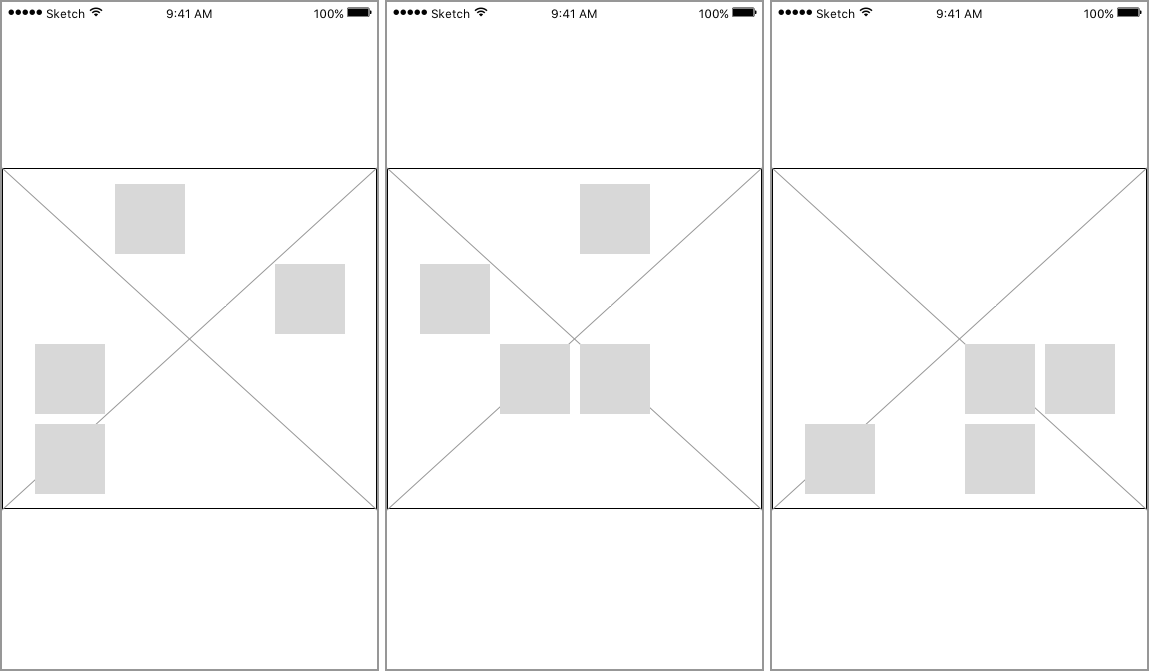
\includegraphics[width=0.45\textwidth]{images/Grid.png}
    \caption{Three examples of the grid as presented over a picture.}~
    \label{fig:grid}
\end{figure}

All the data that was collected was anonymously and securely sent realtime to a Firebase\footnote{\url{http://firebase.google.com/}} database. Firebase utilizes a JSON\footnote{\url{http://www.json.org}} tree structure that can be described as in Figure \ref{fig:datastructure}.
\begin{figure}[h]
    \centering
    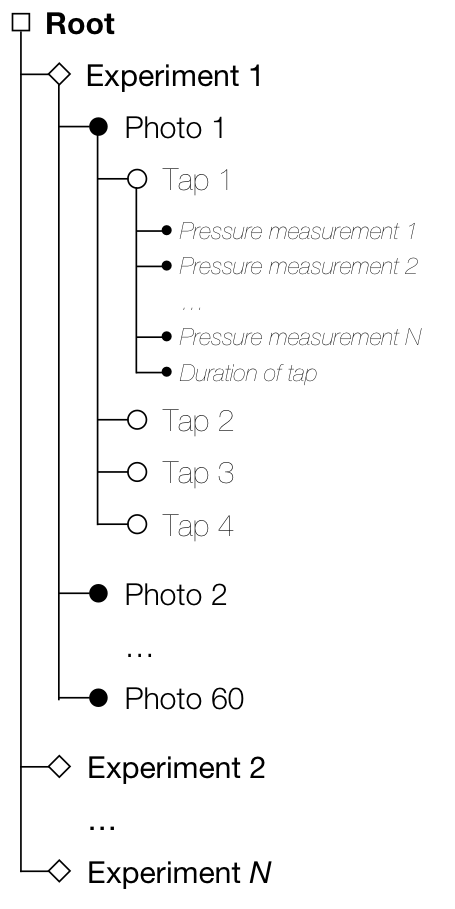
\includegraphics[width=0.3\textwidth]{images/Datastructure.png}
    \caption{Database structure in simplified form.}
    \label{fig:datastructure}
\end{figure}

% subsection data_collection (end)

\subsection{Experiment setup} % (fold)
\label{sub:experiment_setup}
Firstly, participants were told what the expirement entailed and were presented with a consent form. Subsequently, the participants continued the experiment on the smart device with test application. The test application is structured as follows:
\begin{enumerate}
  \item Participant is presented with a screen that asks if they received and signed a consent form and if not, that they should contact the supervisor immediately. There is also a \textit{start} button to start the experiment.
  \item The participant is shown a picture.
  \item After five seconds, four gray buttons are shown, overlaid on the picture in a random pattern (Figure \ref{fig:grid}).
  \item When the participant pressed all the 4 buttons, the next picture is presented.
  \item This process repeats untill al 60 pictures have been shown.
  \item The participant is presented with a conclusive screen that has a thank you message and refers to the supervisor if there are questions.
\end{enumerate}
% subsection experiment_setup (end)

\subsection{Data analysis}
\label{sub:data_analysis}
The collected data was exported as JSON from Firebase and subsequently mutated using Python\footnote{\url{https://www.python.org}} 2.7 on macOS\footnote{\url{https://www.apple.com/lae/macos/sierra/}} 10.12.4 in order to create an \textit{.csv} file that was readable by SPSS 20.0\footnote{\url{https://www.ibm.com/analytics/us/en/technology/spss/}}. Because of a suspiscion that either maximum exerted pressure or average exerted pressure of a tap might be of influence, these two variables were manually added using averaging. For maximum pressure, the maximum pressure value of each tap was extracted, and for each photo this was averaged. Regarding average tap pressure, the average pressure of a tap was calculated and subsequently all the average tap pressures were averaged again per photo. These averages make it possible to compare means. The result is six variables in SPSS; 
\begin{enumerate}
  \item \textbf{Photo filename} - String, containing the photo filename for identification purposes.
  \item \textbf{Valence} - Numeric, decimal value on a scale from 0.0-100.0.
  \item \textbf{Arousal} - Numeric, decimal value on a scale from 0.0-100.0.
  \item \textbf{Maximum tap pressure average} - Numeric, decimal value on scale from 0.0-6.67.
  \item \textbf{Average tap pressure average} - Numeric, decimal value on scale from 0.0-6.67.
  \item \textbf{Duration} - Numeric, decimal value in nanoseconds.
\end{enumerate}

In other words, for every photo there is a value for valence, arousal, maximum tap pressure average, average tap pressure average and duration.

\subsubsection{Multiple linear regression}
\label{subsub:multiple_linear_regression}
Testing for any correlation was completed with a multiple linear regression method. The advantage of this method is that both \textit{duration} and \textit{pressure} can be used as independent variables to check if there indeed is a relation to \textit{valence} or \textit{arousal} as dependent variables and that if there is a relationship, it also immediately produces a model to predict the dependent variables. A disadvantage of is that the relationship can not be checked for \textit{valence} and \textit{arousal} simultaneously, only for the seperate variables.

What follows is four seperate multiple linear regression tests, two with \textit{valence} as dependent variable, and two with \textit{arousal} as dependent variable. Both dependent variables were tested for any relation ship with either \textit{maximum tap pressure \& duration} or \textit{average tap pressure \& duration}.

Before proceeding to the results, several assumptions needed to be considered before concluding that the data could be analysed using multiple linear regression;
\begin{enumerate}
  \item \textbf{Independence of observation} - Using Durbin-Watson to test for 1st-order autocorrelation. Value should be 2 $\pm$0.5.
  \item \textbf{Linear relationships} - Visually inspecting a scatterplot of studentitized residuals and unstandardized predicted values, and partial regression plots can indicate a (non)linear relationship.
  \item \textbf{Homoscedasticity of residuals} - Visually inspecting a scatter plot of studentitized residuals and unstandardized predicted values.
  \item \textbf{No multicollinearity} - Inspection of correlation coefficients and Tolerance/VIF values for indication of correlation between independent variables.
  \item \textbf{No unusual data points} - There should be no outliers, high leverage points or highly influential points.
  \item \textbf{Normal distribution of errors} - Errors in prediction need to be normally distributed, otherwise determining significance can become problematic. By visually inspecting the histogram, Q-Q and P-P plots.
\end{enumerate}
All these assumptions are considered and results of any tests that came with it are presented in the next section.

% \subsubsection{Maximum tap pressure}
% \label{subsub:maximum_tap_pressure}
% The first interpretation regards maximum tap pressure. For every tap, only the maximum pressure value was extracted and subsequently averaged for every photo. This resulted in two independent variables (valence, arousal) and one dependent  variable (average maximum tap force) per photo. A multiple regression was run to predict tap pressure from valence and arousal. An advantage of using the multiple regression for prediction is that during the process, any significant relationships arise.

% \subsubsection{Average tap pressure}
% \label{subsub:average_tap_pressure}
% The procedure for average tap pressure resembled the procedure of maximum tap pressure (Section \ref{subsub:maximum_tap_pressure}), with the only difference being the use of average tap pressure rather than maximum tap pressure, i.e. all pressure measurements of one tap were averaged.



What statistical methods were used, based on what principles and data..

\begin{itemize}
  \item Overview of the research.
  \item Report of who took part and where.
  \item Report of what procedures were used.
  \item Report of what materials were used.
  \item Report of any statistical analysis used.
\end{itemize}

% section methods (end)

\section{Results} % (fold)
\label{sec:results}
\begin{itemize}
  \item Report of findings.
  \item Reference to any diagrams used.
\end{itemize}

In this section, results of the measurements are presented. It starts with 

First, the results of \textit{maximum tap pressure} and \textit{duration} are presented. Secondly, \textit{average tap pressure} and \textit{duration}. Subsequently,

\subsection{Assumptions}
\label{sub:assumptions}

\subsubsection{Independence of observation}
As can be seen in Table \ref{tab:durbin_watson}, the Durbin-Watson values exceed acceptable limits for each seperate test, indicating a strong positive autocorrelation. However, Durbin-Watson is used for time-series data. Since the collected data is not a time-series, the positive autocorrelation can be safely ignored.
%!TEX root = ../Thesis.tex
\begin{table}[]
\centering
\begin{tabular}{@{}llr@{}}
\textbf{Dependent variable} & \textbf{Independent variables} & \textbf{d-w} \\ \midrule
Valence                     & Max. tap pressure, duration  & .567         \\ 
                            & Avg. tap pressure, duration  & .570         \\ \midrule
Arousal                     & Max. tap pressure, duration  & .847         \\ 
                            & Avg. tap pressure, duration  & .858        
\end{tabular}
\caption{Durbin-Watson values (d-w) outside of $2 \pm 0.5$ indicate autocorrelation issues.}
\label{tab:durbin_watson}
\end{table}

\subsubsection{Linear relationships}
By visually inspecting scatter plots of the \textit{unstandardized predicted value} against \textit{studentized residuals} it can be assumed there is linearity. Furthermore, by looking at partial regression plots of each of the independent variables for every dependent variable, it is again apparent that there is an approximate linear relationship. See Appendix Linear Relationships and Homoscedasticity for the graphs used for inspection.

\subsubsection{Homoscedasticity}
Using the scatter plots of \textit{unstandardized predicted value} against \textit{studentized residuals} for inspection, the random spread of values indicate homoscedasticity of values. See Appendix Linear Relationships and Homoscedasticity for the graphs used for inspection.

\subsubsection{Multicollinearity}
Inspection of correlation coefficients (Appendix Multicollinearity for full tables) show none of the correlations $> 0.7$. In Table \ref{tab:collinearity_tolerance}, tolerance values are found. None of the tolerance values fall below the limit of $0.1$
%!TEX root=../Thesis.tex
\begin{table}[]
\centering
\begin{tabular}{@{}llr@{}}
\textbf{Dependent variable} & \textbf{Independent variables} & \textbf{Tolerance} \\ \midrule
Valence                     & Maximum tap pressure           & .728               \\
                            & Duration                       & .728               \\ \cmidrule(l){2-3} 
                            & Average tap pressure           & .758               \\
                            & Duration                       & .758               \\ \midrule
Arousal                     & Maximum tap pressure           & .728               \\
                            & Duration                       & .728               \\ \cmidrule(l){2-3} 
                            & Average tap pressure           & .758               \\
                            & Duration                       & .758              
\end{tabular}
\caption{Tolerance values $< 0.1$ indicate collinearty issues.}
\label{tab:collinearity_tolerance}
\end{table}

\subsection{Unusual data points} % (fold)
\label{sub:unusual_data_points}

% subsection unusual_data_points (end)

\subsection{Maximum tap pressure}
There was linearity as assessed by partial regression plots and a plot of studentized residuals against the predicted values. There was independence of residuals, as assessed by a Durbin-Watson statistic of 1.718. There was homoscedasticity, as assessed by visual inspection of a plot of studentized residuals versus unstandardized predicted values. There was no evidence of multicollinearity, as assessed by tolerance values greater than 0.1. There were no studentized deleted residuals greater than $\pm$3 standard deviations, no leverage values greater than 0.2, and values for Cook's distance above 1. The assumption of normality was met, as assessed by Q-Q Plot. The multiple regression model did not statistically significantly predicted tap pressure, $F(2, 57) = 2.033$, $p > 0.05$, adj. $R^2$ = 0.034. Non of the variables added statistically significantly to the prediction(i.e. $p > 0.05$), with $p_{valence} = 0.35$ and $p_{arousal} = 0.079$. %Regression coefficients and standard errors can be found in Table \ref{tab:summary_multiple_regression_max_pressure_avg}.

% Coefficients are not interesting if there is no significance, they are only used for prediction models.
% \begin{table}[ht]
% \centering
%   \begin{threeparttable}
%     \caption{Summary of multiple regression analysis for maximum pressure average.\label{tab:summary_multiple_regression_max_pressure_avg}}
%     \begin{tabularx}{0.9\linewidth}{@{}lYYY@{}}
%       \toprule
%       Variable  & \textit{B} & \textit{$SE_{B}$} & \textit{$\beta$} \\ \midrule
%       Intercept & .375       & .024              &                  \\
%       Valence   & .000       & .000              & .213             \\
%       Arousal   & .001       & .000              & .403             \\ \bottomrule
%     \end{tabularx}
%   \begin{tablenotes}
%     \small
%     \item Note: \textit{B} = unstandardized regression coefficient. \textit{$SE_B$} = Standard error of the coefficient. $\beta$ = standardized coefficient.
%   \end{tablenotes}
%   \end{threeparttable}
% \end{table}
% section results (end)

\section{Discussion} % (fold)
\label{sec:discussion}
\begin{itemize}
  \item Summary of main purpose of research.
  \item Review of most important findings.
  \item Evaluation of findings.
  \item Explanation of findings.
  \item Comparison with other researchers findings.
  \item Description of implications and recommendations.
\end{itemize}


% section discussion (end)


% REFERENCES FORMAT
% References must be the same font size as other body text.
\bibliographystyle{SIGCHI-Reference-Format}
\bibliography{library,Alternative}
\clearpage
\onecolumn

% Start of appendices
\appendix
\section{Linear relationships and homoscedasticity}
\label{app:linear_relationships}

\subsection{Scatter plot: unstandardized predicted value vs. studentized residuals}
\hfill \break
%!TEX root = ../Thesis.tex
\begin{figure}[h]
\centering
\begin{subfigure}[b]{0.45\textwidth}
    \centering
    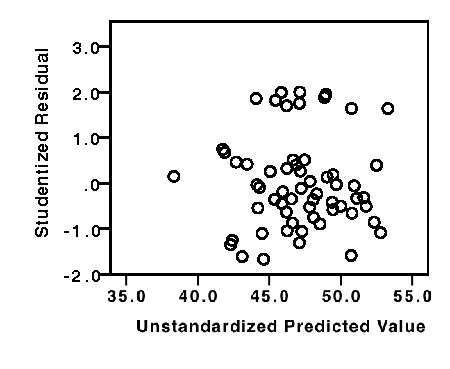
\includegraphics[width=\textwidth]{images/linearity/ValMax.eps}
    \caption{Related to test of valence, maximum pressure, and duration}
    \label{fig:valence_maximum}
\end{subfigure}
\quad
\begin{subfigure}[b]{0.45\textwidth}
    \centering
    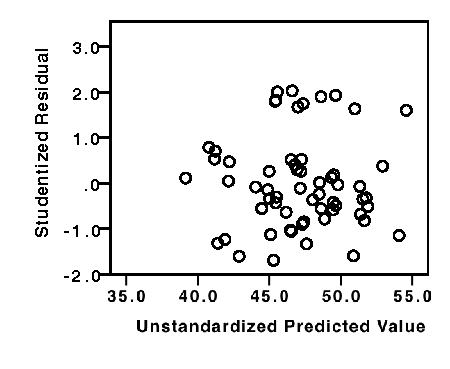
\includegraphics[width=\textwidth]{images/linearity/ValAvg.eps}
    \caption{Related to test of valence, average pressure, and duration}
    \label{fig:valence_avg}
\end{subfigure}
\par\bigskip
\par\bigskip
\begin{subfigure}[b]{0.45\textwidth}
    \centering
    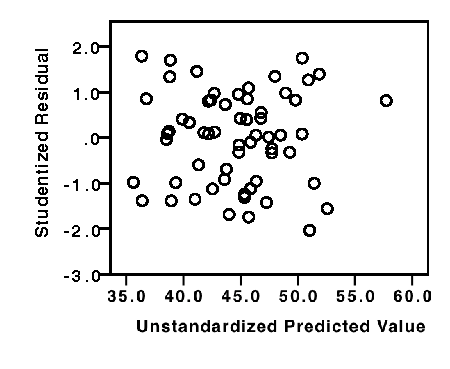
\includegraphics[width=\textwidth]{images/linearity/ArMax.eps}
    \caption{Related to test of arousal, maximum pressure, and duration}
    \label{fig:arousal_maximum}
\end{subfigure}
\quad
\begin{subfigure}[b]{0.45\textwidth}
    \centering
    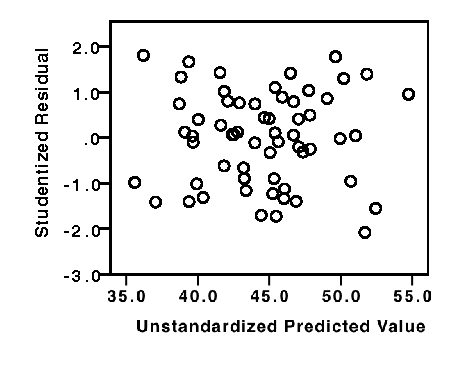
\includegraphics[width=\textwidth]{images/linearity/ArAvg.eps}
    \caption{Related to test of arousal, average pressure, and duration}
    \label{fig:arousal_avg}
\end{subfigure}
\caption{Scatter plots of predicted values against studentitized residuals. Note that because of random nature, linearity can still be assumed.}
\end{figure}
\clearpage

\subsection{Partial regression plots}
\hfill \break
%!TEX root = ../Thesis.tex
\begin{figure}[ht]
  \centering
  \begin{subfigure}[b]{0.45\textwidth}
    \centering
    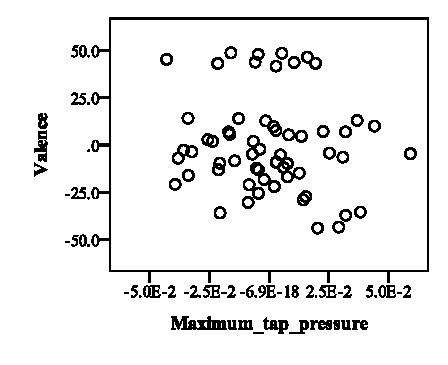
\includegraphics[width=\textwidth]{images/linearity/partialregression/valence/ValMaxMax.eps}
    \label{fig:valmaxmax}
  \end{subfigure}
  \quad
  \begin{subfigure}[b]{0.45\textwidth}
    \centering
    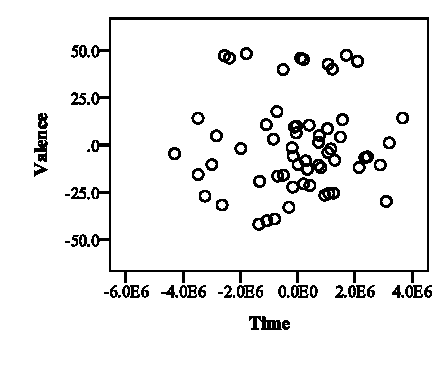
\includegraphics[width=\textwidth]{images/linearity/partialregression/valence/ValMaxTime.eps}
    \label{fig:valmaxtime}
  \end{subfigure}
  \caption{Partial regression plots with valence (dependent variable), maximum pressure and duration (independent variables). Note the approximate linearity.}
\end{figure}

\begin{figure}[ht]
  \centering
  \begin{subfigure}[b]{0.45\textwidth}
    \centering
    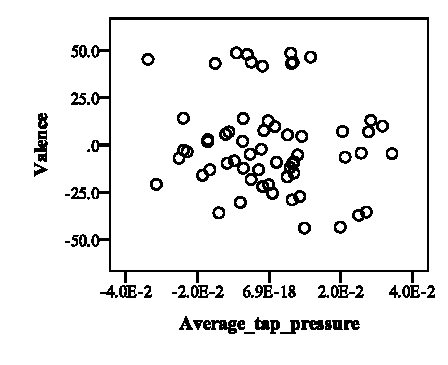
\includegraphics[width=\textwidth]{images/linearity/partialregression/valence/ValAvgAvg.eps}
    \label{fig:valavgavg}
  \end{subfigure}
  \quad
  \begin{subfigure}[b]{0.45\textwidth}
    \centering
    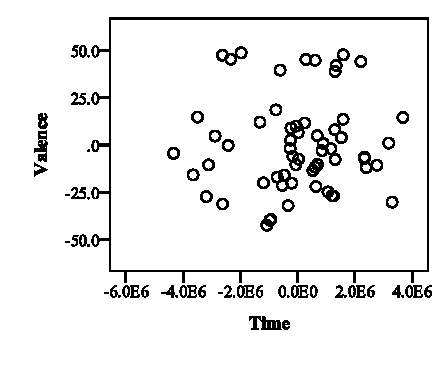
\includegraphics[width=\textwidth]{images/linearity/partialregression/valence/ValAvgTime.eps}
    \label{fig:valavgtime}
  \end{subfigure}
  \caption{Partial regression plots with valence (dependent variable), average pressure and duration (independent variables). Note the approximate linearity.}
\end{figure}
%!TEX root = ../Thesis.tex
\begin{figure}[ht]
  \centering
  \begin{subfigure}[b]{0.45\textwidth}
    \centering
    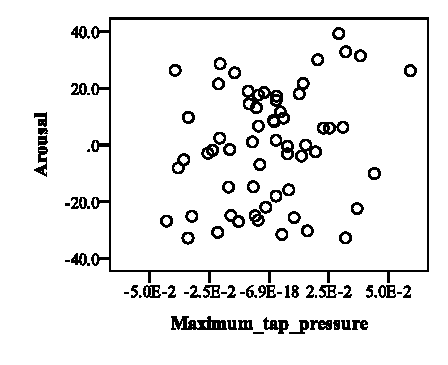
\includegraphics[width=\textwidth]{images/linearity/partialregression/arousal/ArMaxMax.eps}
    \label{fig:armaxmax}
  \end{subfigure}
  \quad
  \begin{subfigure}[b]{0.45\textwidth}
    \centering
    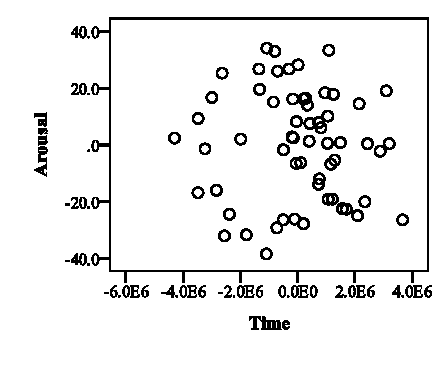
\includegraphics[width=\textwidth]{images/linearity/partialregression/arousal/ArMaxTime.eps}
    \label{fig:armaxtime}
  \end{subfigure}
  \caption{Partial regression plots with arousal (dependent variable), maximum pressure and duration (independent variables). Note the approximate linearity.}
\end{figure}

\begin{figure}[ht]
  \centering
  \begin{subfigure}[b]{0.45\textwidth}
    \centering
    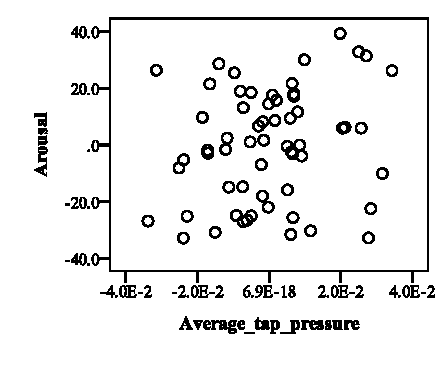
\includegraphics[width=\textwidth]{images/linearity/partialregression/arousal/ArAvgAvg.eps}
    \label{fig:aravgavg}
  \end{subfigure}
  \quad
  \begin{subfigure}[b]{0.45\textwidth}
    \centering
    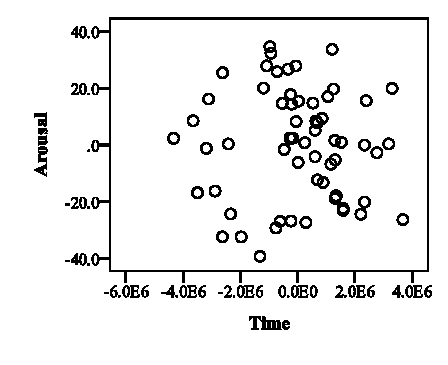
\includegraphics[width=\textwidth]{images/linearity/partialregression/arousal/ArAvgTime.eps}
    \label{fig:aravgtime}
  \end{subfigure}
  \caption{Partial regression plots with arousal (dependent variable), average pressure and duration (independent variables). Note the approximate linearity.}
\end{figure}
\clearpage

\section{Multicollinearity} % (fold)
\label{app:multicollinearity}
\hfill \break
%!TEX root=../Thesis.tex
\begin{table}[ht]
\centering
\begin{tabular}{@{}llrrr@{}}
                    &                   & Valence & Duration & Max. tap pressure \\ \midrule
Pearson Correlation & Valence           & 1.000   & -.028    & -.120             \\
                    & Duration          & -.028   & 1.000    & .522              \\
                    & Max. tap pressure & -.120   & .522     & 1.000             \\ \midrule
Sig. (1-tailed)     & Valence           & .       & .415     & .181              \\
                    & Duration          & .415    & .        & .000              \\
                    & Max. tap pressure & .181    & .000     & .                
\end{tabular}
\caption{Correlations of valence, maximum tap pressure and duration.}
\label{tab:correlations_valmax}
\end{table}

\par\bigskip

\begin{table}[ht]
\centering
\begin{tabular}{@{}llrrr@{}}
                    &                   & Valence & Duration & Avg. tap pressure \\ \midrule
Pearson Correlation & Valence           & 1.000   & -.028    & -.132             \\
                    & Duration          & -.028   & 1.000    & .492              \\
                    & Avg. tap pressure & -.132   & .492     & 1.000             \\ \midrule
Sig. (1-tailed)     & Valence           & .       & .415     & .158              \\
                    & Duration          & .415    & .        & .000              \\
                    & Avg. tap pressure & .158    & .000     & .                
\end{tabular}
\caption{Correlations of valence, average tap pressure and duration}
\label{tab:correlations_valavg}
\end{table}

\par\bigskip

\begin{table}[ht]
\centering
\begin{tabular}{@{}llrrr@{}}
                    &                   & Arousal & Duration & Max. tap pressure \\ \midrule
Pearson Correlation & Arousal           & 1.000   & .080     & .228              \\
                    & Duration          & .080    & 1.000    & .522              \\
                    & Max. tap pressure & .228    & .522     & 1.000             \\ \midrule
Sig. (1-tailed)     & Arousal           & .       & .272     & .040              \\
                    & Duration          & .272    & .        & .000              \\
                    & Max. tap pressure & .040    & .000     & .                
\end{tabular}
\caption{Correlations of arousal, maximum tap pressure and duration}
\label{tab:correlations_armax}
\end{table}

\par\bigskip

\begin{table}[!htbp]
\centering
\begin{tabular}{@{}llrrr@{}}
                    &                   & Arousal & Duration & Avg. tap pressure \\ \midrule
Pearson Correlation & Arousal           & 1.000   & .080     & .212              \\
                    & Duration          & .080    & 1.000    & .492              \\
                    & Avg. tap pressure & .212    & .492     & 1.000             \\ \midrule
Sig. (1-tailed)     & Arousal           & .       & .272     & .052              \\
                    & Duration          & .272    & .        & .000              \\
                    & Avg. tap pressure & .052    & .000     & .                
\end{tabular}
\caption{Correlations of arousal, average tap pressure and duration}
\label{tab:correlations_aravg}
\end{table}
\clearpage
% section multicollinearity (end)


\end{document}

%%% Local Variables:
%%% mode: latex
%%% TeX-master: t
%%% End:
